\documentclass[nobib]{tufte-handout}

\title{Lecture 11: Planarity $\cdot$ 1MA020}

\author[Vilhelm Agdur]{Vilhelm Agdur\thanks{\href{mailto:vilhelm.agdur@math.uu.se}{\nolinkurl{vilhelm.agdur@math.uu.se}}}}

\date{20 November 2023}


%\geometry{showframe} % display margins for debugging page layout

\usepackage{graphicx} % allow embedded images
  \setkeys{Gin}{width=\linewidth,totalheight=\textheight,keepaspectratio}
  \graphicspath{{graphics/}} % set of paths to search for images
\usepackage{amsmath}  % extended mathematics
\usepackage{booktabs} % book-quality tables
\usepackage{units}    % non-stacked fractions and better unit spacing
\usepackage{multicol} % multiple column layout facilities
\usepackage{lipsum}   % filler text
\usepackage{fancyvrb} % extended verbatim environments
  \fvset{fontsize=\normalsize}% default font size for fancy-verbatim environments

\usepackage{color,soul} % Highlights for text

% Standardize command font styles and environments
\newcommand{\doccmd}[1]{\texttt{\textbackslash#1}}% command name -- adds backslash automatically
\newcommand{\docopt}[1]{\ensuremath{\langle}\textrm{\textit{#1}}\ensuremath{\rangle}}% optional command argument
\newcommand{\docarg}[1]{\textrm{\textit{#1}}}% (required) command argument
\newcommand{\docenv}[1]{\textsf{#1}}% environment name
\newcommand{\docpkg}[1]{\texttt{#1}}% package name
\newcommand{\doccls}[1]{\texttt{#1}}% document class name
\newcommand{\docclsopt}[1]{\texttt{#1}}% document class option name
\newenvironment{docspec}{\begin{quote}\noindent}{\end{quote}}% command specification environment

\include{mathcommands.extratex}

\begin{document}

\maketitle% this prints the handout title, author, and date

\begin{abstract}
\noindent
We study the notion of a graph being \emph{planar}, define its \emph{planar dual}, and prove some results about when a graph is planar. We give most of a proof of the theorems of Kuratowski and Wagner about forbidden minors for planar graphs. Finally, we introduce the notion of outerplanar graphs.
\end{abstract}

\section{Three-connected graphs}

While the topic of this lecture is planarity, we will need a result about the structure of three-connected graphs. So we begin by proving this.

\begin{figure}
  \centering
  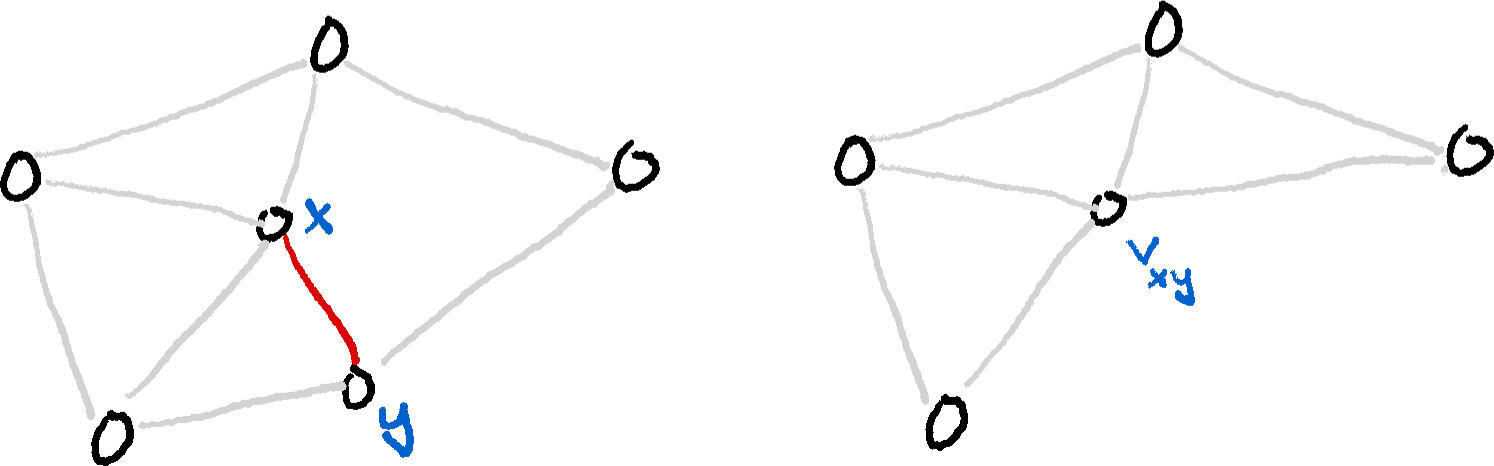
\includegraphics[width=0.75\textwidth]{graphics/L10_connectivity/edge_contraction.png}
  \caption[][0cm]{A graph with an edge between $x$ and $y$ highlighted in red. On the right, the result of contracting this edge.}
  \label{fig:edge_contraction}
\end{figure}

\begin{definition}
  Let $G = (V,E)$ be a graph and $e = x\sim y$ be an edge of $G$. The \emph{contraction} of $e$ is the graph $G/e$, which we construct as follows:

  Introduce a new vertex $v_{xy}$, and let $V(G/e) = (V \setminus \{x,y\}) \cup \{v_{xy}\}$. Replace each edge $w \sim x$ or $w \sim y$ with an edge $w \sim v_{xy}$.
\end{definition}

\begin{lemma}
  If $G = (V,E)$ is three-connected and has more than four vertices, then there exists an edge $e \in E$ such that $G/e$ is again three-connected.

  \begin{proof}
    Suppose there is no such edge, so that for every edge $e = x \sim y$ there is a separating set $X$ of $G/e$ on two or fewer vertices. Now, since $G$ is three-connected, we must in fact have $X = \{v_{xy}, z\}$.

    Then the set $\{x, y, z\}$ must be a separating set for $G$. Each of these three vertices must have a neighbour in every connected component of $G[V \setminus \{x,y,z\}]$.\sidenote[][]{
      \begin{xca}
        Prove this.
      \end{xca}
    } Let $C$ be the smallest such component, and further assume we chose $x$, $y$, and $z$ in such a way that $\abs{V(C)}$ was minimal across all choices.

    Now, choose a neighbour $v$ of $z$ in $C$. By our assumption, no edge-contracton is three-connected, so in particular $G/(v \sim z)$ is not three-connected. By entirely the same argument as before, we can find a vertex $w$ such that $\{z,v,w\}$ separates $G$.

    Again, each of $z$, $v$, and $w$ has a neighbour in each connected component of $G[V \setminus \{z, v, w\}]$. Since there is an edge between $x$ and $y$, they must be in the same component, and so there is a component $D$ which contains neither. Since $v \in C$, each of its neighbours is also in $C$, and so in particular is its neighbour in $D$.

    So $D \cap C \neq \emptyset$. Since $D$ does not contain any of $x$, $y$, or $z$, their removal can't disconnect $D$, and so it follows from this that $D \subseteq C$. However, $D$ clearly does not contain $v$, being a connected component of $G[V \setminus \{z, v, w\}]$, while $C$ does contain $v$. So $D$ is in fact strictly smaller than $C$, which is a contradiction, since we assumed $C$ was minimal. So the lemma follows.
  \end{proof}
\end{lemma}

For our final theorem, we do not offer a proof, just a statement. It is in some sense analogous to our theorem about two-connected graphs being constructible by adding paths to a cycle graph.

\begin{theorem}[Tutte, 1961]
  A graph $G$ is three-connected if and only if there exists a sequence $G_0, G_1,\ldots, G_n$ of graphs, where $G_0 = K_4$, $G_n = G$, and for every $i \in [n]$ the graph $G_i$ has an edge $u \sim v$ with $d_{G_i}(u), d_{G_i}(v) \geq 3$ and $G_{i-1} = G_i/(u\sim v)$.
\end{theorem}

\section{Exercises}


%\bibliography{references}
%\bibliographystyle{plainnat}

\end{document}
